\begin{figure}[H]
	\centering
	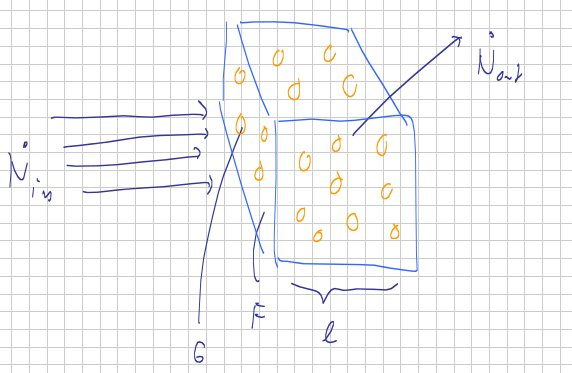
\includegraphics[width=0.5\textwidth]{wq.jpg}
	\caption{	 ???}
	\label{wq}
\end{figure}


\[ N_T = \frac{\rho\cdot V}{A}\cdot N_A~~~~~~ \text{mit}~~~~~ \rho
\left[\frac{\text{g}}{\text{cm}^3} \right],~~~A\left[\frac{\text{g}}{\text{mol}} \right],~~~N_A\left[\text{mol}^{-1} \right] \] 

Teilchendichte: $n=\frac{N_T}{V}=\frac{\rho}{A}\cdot N_A$

Der einfliegende Strahl sieht eine $N_T\cdot\sigma$-große Fläche. Die
Wechselwirkungswahrscheinlichkeit ist daher

\[w= \frac{N_T\cdot\sigma}{F} = \frac{\dot{N}_\text{out}}{\dot{N}_\text{in}} = n\cdot \sigma \cdot
l. \]

Damit ergibt sich der Wirkungsquerschnitt zu 

\[\sigma =\frac{\dot{N}_\text{out}}{\dot{N}_\text{in}}\cdot \frac{1}{n\cdot l} . \]

Es kommt zu einem exponentiellen Abfall für Teilchen, die keine Reaktion mit dem Target hatten:

\[\frac{\mathrm{d}N}{N} = -n\cdot \sigma\cdot \mathrm{d} x ~~~\Rightarrow~~~ N(x)=N_0\cdot
e^{-\alpha x}
\]

mit $\alpha=n\cdot \sigma$. Für die mittlere freie Weglänge folgt

\[\lambda =\frac{1}{n\cdot\sigma}=\frac{1}{\alpha}.  \]

Als Beispiel eine Abschätzung für hadronische Wechselwirkung (Nukleon $+X$):

\[\sigma = \pi\cdot r_p^2 = 30\,\text{mb} \]

pro Nukleon. Für ganze Atomkerne folgt dann

\[\sigma_\text{Atomkern} \approx (30-50)\,\text{mb}\cdot A^{2/3}\]
